\makeatletter
\def\input@path{{../}}
\makeatother
\documentclass[../master_thesis.tex]{subfiles}
\begin{document}
\chapter{Results}\label{chap:Results}
\section{Overview of Tests}
We divided the tests of this implementation into four main types, theoretical
correctness, parametrization, comparizon and tests of the variational implementation.

In the tests of theoretical correctness we test if our implementation gives the
results to problems as expected. The tests for this were comparisons to
the energy of  \ce{Li^+} in an environment with dielectric constant $\epsinf = 2$
with the value we would get from the Born model. In the Born model the energy of a  %citation please
one atom ion in a solvent is the same as the energy of a point charge in the same solvent.
This energy is described as
\begin{equation}
  E_{ion} = -\frac{q^{2}}{8 \pi a}\left(\frac{1}{\epsilon_{0}}-\frac{1}{\epsilon}\right)
\end{equation}
A second comparizon with the born model was done where we tested for the
following relation that should hold for a point charge
\begin{equation}
  \int \gamma_s = \frac{\epsinf - 1}{\epsinf} q
\end{equation}

The parametrization tests were done by changing one parameter at a time while
comparing this same change to Gaussian calculations with different basis sets.
First we only checked the dependency on the radius and how changing it would
affect the reaction field energy with respect to Gaussian calculations of the same
radii. We the compared Gaussian calculations of Radius $R$ against \mrchem
calculations of Radius $R+0.2$ in an attempt to see an improvement in the
results.
A second parametrization test was done with was doen with only \ce{Li^+}
where we changed the relative precision of the \mrchem calculations to see how
they would affect the energy with respect to the Gaussian energies. This as well
was done on different radii.

We then took 4 molecules that were tested by \cite{Chipman2002} and compared the
results from variation of radii against Gaussian results. THis was done for both
single sphere cavities and for \ac{ABC}.

Lastly we tested out variational principle with water and \ce{Li^+}.


\section{Data}
\subsection{\ac{ABC} tests}
The data tables containing all results can be found at the end of the chapter in section \ref{Datatables}, following
tables will show a small sample so the reader can make better understand the tables
in the appendixes.

The following table \ref{tab:rawwaterdata}  presents the data for the energy
calculations of \ce{H_2O} with the three first cavity radii as an example.
These are the total \ac{SCF} energy values.
The same type of tables were used for the rest of the
systems.
\begin{table}[htbp]
\caption{Total Energy Calculations example for Water in Water. Energy in Hartree and radii of the cavity in Bohr}
\begin{center}
\begin{tabular}{|l|r|r|r|r|}
\hline
Basis & $R =3.6$ & $R=3.7$ & $R=3.8$ & $\ldots$\\  \hline
Cc-pVDZ & -7.6039e+01 & -7.6038e+01 & -7.6036e+01 & $\ldots$\\ \hline
Cc-pVTZ & -7.6070e+01 & -7.6069e+01 & -7.6067e+01 & $\ldots$\\ \hline
Cc-pVQZ & -7.6078e+01 & -7.6076e+01 & -7.6075e+01 & $\ldots$\\ \hline
Cc-pV5Z & -7.6080e+01 & -7.6079e+01 & -7.6077e+01 & $\ldots$\\ \hline
Aug-cc-pVDZ & -7.6054e+01 & -7.6053e+01 & -7.6052e+01 & $\ldots$\\ \hline
Aug-cc-pVTZ & -7.6074e+01 & -7.6072e+01 & -7.6071e+01 & $\ldots$\\ \hline
Aug-cc-pVQZ & -7.6079e+01 & -7.6077e+01 & -7.6076e+01 & $\ldots$\\ \hline
Aug-cc-pV5Z & -7.6080e+01 & -7.6079e+01 & -7.6077e+01 & $\ldots$\\ \hline
daug-cc-pVDZ & -7.6055e+01 & -7.6053e+01 & -7.6052e+01 & $\ldots$\\ \hline
daug-cc-pVTZ & -7.6074e+01 & -7.6072e+01 & -7.6071e+01 & $\ldots$\\ \hline
daug-cc-pVQZ & -7.6079e+01 & -7.6077e+01 & -7.6076e+01 & $\ldots$\\ \hline
daug-cc-pV5Z & -7.6080e+01 & -7.6079e+01 & -7.6077e+01 & $\ldots$\\ \hline
mrchem & -7.6085E+01 & -7.6083E+01 & -7.6081E+01 & $\ldots$\\ \hline
\end{tabular}
\end{center}
\label{tab:rawwaterdata}
\end{table}

In order to get the Reaction field
energies $E_r$ one needs the gas state Energy $E_{vac}$ for a given
basis set and subtract it from the total solvent energy $E_{tot}$ calculated for
that basis set.
\begin{equation}
  E_r = E_{tot} - E_{vac}
\end{equation}
Examples for the first three radii for the results of the above operation can be
seen in table \ref{tab:Erwatdata}

\begin{table}[htbp]
\caption{Reaction Field Energy Calculations example for Water in Water. Energy in Hartree and radii of the cavity in Bohr}
\begin{center}
\begin{tabular}{|l|r|r|r|r|}
\hline
basis & 3.6 & 3.7 & 3.8 & $\ldots$\\ \hline
Cc-pVDZ & -1.2450E-02 & -1.0998E-02 & -9.7804E-03 & $\ldots$\\ \hline
Cc-pVTZ & -1.3097E-02 & -1.1545E-02 & -1.0243E-02 & $\ldots$\\ \hline
Cc-pVQZ & -1.3218E-02 & -1.1651E-02 & -1.0334E-02 & $\ldots$\\ \hline
Cc-pV5Z & -1.3284E-02 & -1.1713E-02 & -1.0393E-02 & $\ldots$\\ \hline
Aug-cc-pVDZ & -1.3190E-02 & -1.1634E-02 & -1.0328E-02 & $\ldots$\\ \hline
Aug-cc-pVTZ & -1.3238E-02 & -1.1670E-02 & -1.0353E-02 & $\ldots$\\ \hline
Aug-cc-pVQZ & -1.3221E-02 & -1.1655E-02 & -1.0338E-02 & $\ldots$\\ \hline
Aug-cc-pV5Z & -1.3223E-02 & -1.1655E-02 & -1.0337E-02 & $\ldots$\\ \hline
daug-cc-pVDZ & -1.3228E-02 & -1.1665E-02 & -1.0351E-02 & $\ldots$\\ \hline
daug-cc-pVTZ & -1.3243E-02 & -1.1675E-02 & -1.0357E-02 & $\ldots$\\ \hline
daug-cc-pVQZ & -1.3223E-02 & -1.1656E-02 & -1.0340E-02 & $\ldots$\\ \hline
daug-cc-pV5Z & -1.3224E-02 & -1.1655E-02 & -1.0337E-02 & $\ldots$\\ \hline
mrchem & -1.8036E-02 & -1.5494E-02 & -1.3437E-02 & $\ldots$\\ \hline
\end{tabular}
\end{center}
\label{tab:Erwatdata}
\end{table}

Following are figures \ref{fig:watEnergyplots},
\ref{fig:nopEnergyplots} and \ref{fig:cyanEnergyplots}
that show the energies of the mrchem calculations plotted
against the energies from the Gaussian calculation for water, \ce{NO^+}, and
\ce{CN^-} respectively. Many of the Mrchem results for \ce{CN^-} and \ce{NO^+}
around the interval $(4.0, 4.5)$ diverged and finished or never finished
running due to divergence, due to this these results were removed from the figures so as to facilitate
the visualization of the trends across the radii. The values which deverged but still
finished running can be viewed in section \ref{Datatables}.

\begin{figure}[h!]
  \centering
  \begin{subfigure}[b]{0.75\linewidth}
    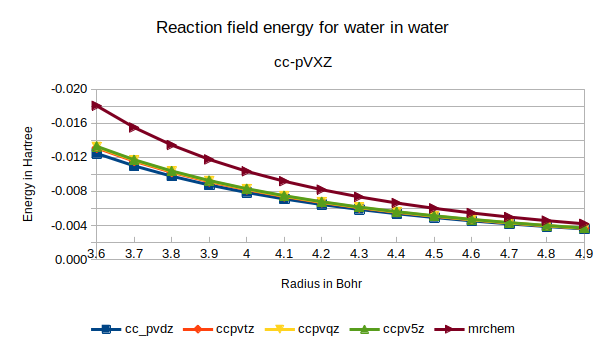
\includegraphics[width=\linewidth]{img/Erwat.png}
  \end{subfigure}
  \begin{subfigure}[b]{0.75\linewidth}
    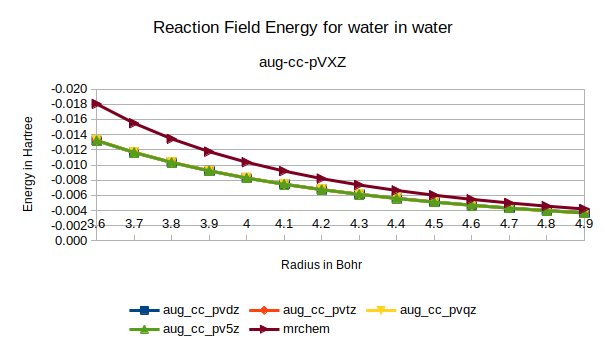
\includegraphics[width=\linewidth]{img/Eraugwat.png}
  \end{subfigure}
  \begin{subfigure}[b]{0.75\linewidth}
    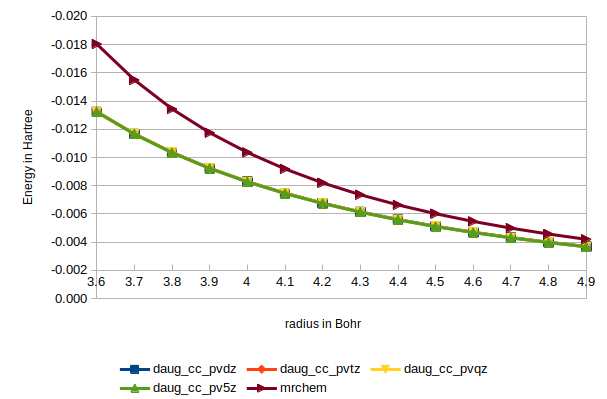
\includegraphics[width=\linewidth]{img/Erdaugwat.png}
  \end{subfigure}
  \caption{Reaction field energy of Water in a water solution, calculated with mrchem
  and with different basis sets in Gaussian}
  \label{fig:watEnergyplots}
\end{figure}

\begin{figure}[h!]
  \centering
  \begin{subfigure}[b]{\linewidth}
    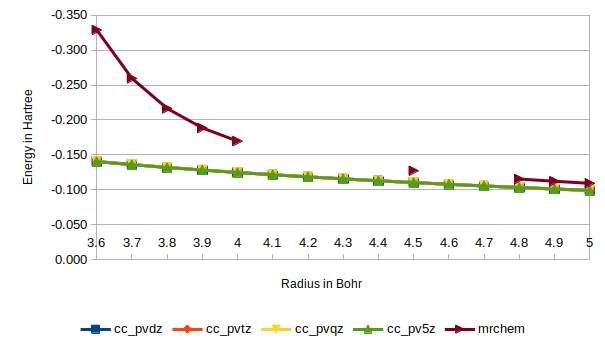
\includegraphics[width=\linewidth]{img/Ernop.png}
  \end{subfigure}
  \begin{subfigure}[b]{\linewidth}
    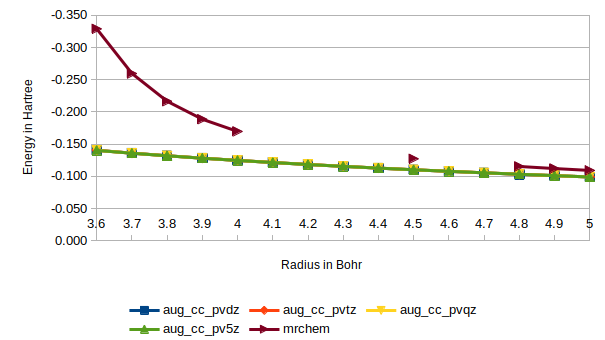
\includegraphics[width=\linewidth]{img/Eraugnop.png}
  \end{subfigure}
  \begin{subfigure}[b]{\linewidth}
    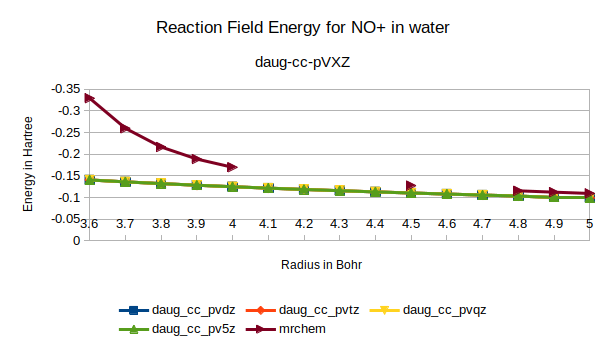
\includegraphics[width=\linewidth]{img/Erdaugnop.png}
  \end{subfigure}
  \caption[Energy plots for \ce{NO^+}]{Reaction field energy of \ce{NO^+} in a water solution, calculated with mrchem
  and with different basis sets in Gaussian}
  \label{fig:nopEnergyplots}

\end{figure}
\begin{figure}[h!]
  \centering
  \begin{subfigure}[b]{\linewidth}
    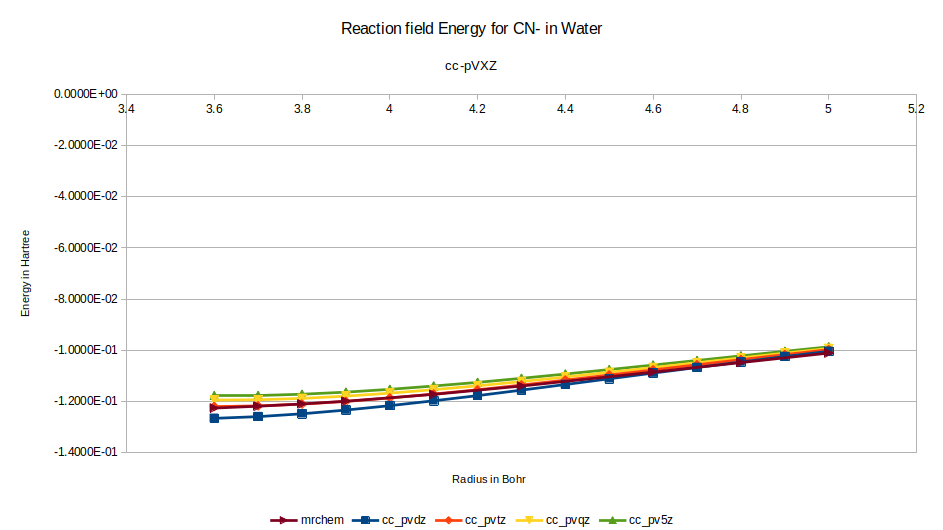
\includegraphics[width=\linewidth]{img/Ercyan.png}
  \end{subfigure}
  \begin{subfigure}[b]{\linewidth}
    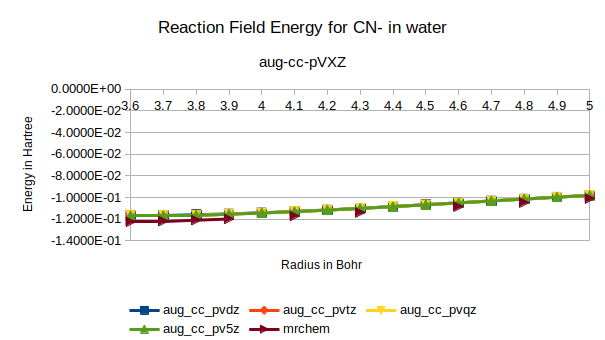
\includegraphics[width=\linewidth]{img/Eraugcyan.png}
  \end{subfigure}
  \begin{subfigure}[b]{\linewidth}
    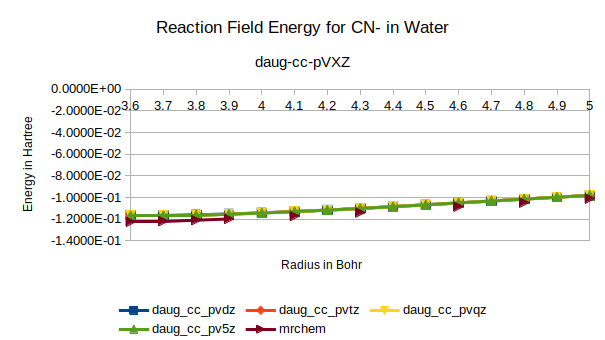
\includegraphics[width=\linewidth]{img/Erdaugcyan.png}
  \end{subfigure}
  \caption{Reaction field energy of \ce{CN^-} in a water solution, calculated with mrchem
  and with different basis sets in Gaussian}
  \label{fig:cyanEnergyplots}
\end{figure}

The Mrchem energy values $E_{Mrchem}$ for each radii were compared to the
corresponding values of each of the different basis set calculations in
Gaussian  $E_{Gaussian}^{basis}$ by finding the relative difference $d_r$
between them as
\begin{equation}\label{eq:reldiff}
  d_r = \frac{E_{Gaussian}^{basis} - E_{Mrchem}}{E_{Mrchem}}
\end{equation}
The operation above \ref{eq:reldiff} was applied to all the values for all the
substrate molecules, giving the following figures \ref{fig:watreldiff},
\ref{fig:nopreldiff}, and \ref{fig:cyanreldiff}.

\begin{figure}[h!]
  \centering
  \begin{subfigure}[b]{\linewidth}
    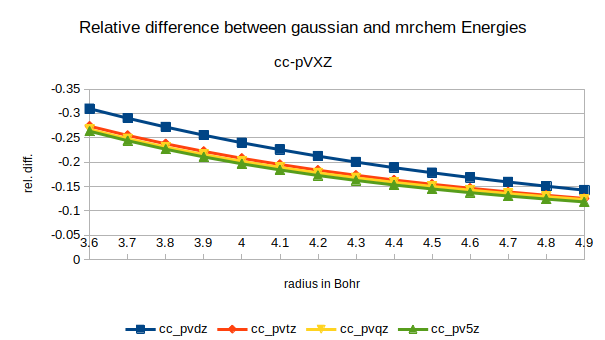
\includegraphics[width=\linewidth]{img/watreldiff.png}
  \end{subfigure}
  \begin{subfigure}[b]{\linewidth}
    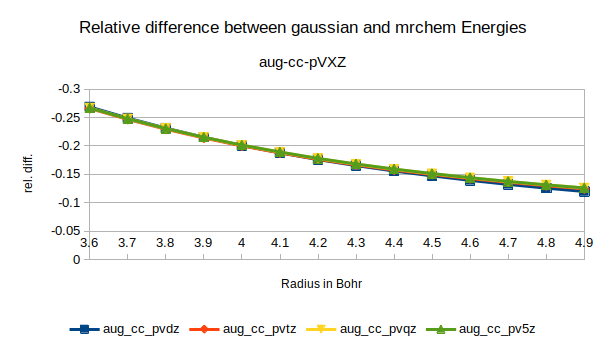
\includegraphics[width=\linewidth]{img/wataugreldiff.png}
  \end{subfigure}
  \begin{subfigure}[b]{\linewidth}
    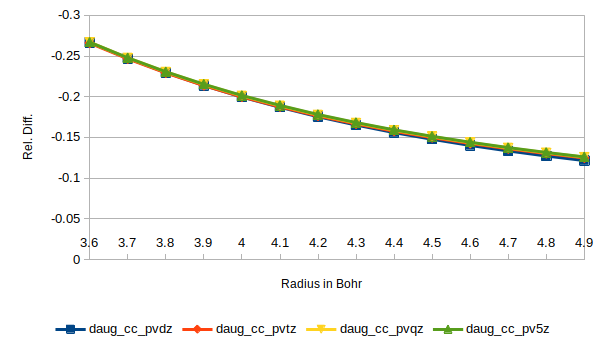
\includegraphics[width=\linewidth]{img/watdaugreldiff.png}
  \end{subfigure}
  \caption{Relative difference between the Reaction field energy of Water in a water solution calculated with mrchem
  and with different basis sets in Gaussian}
  \label{fig:watreldiff}
\end{figure}

\begin{figure}[h!]
  \centering
  \begin{subfigure}[b]{\linewidth}
    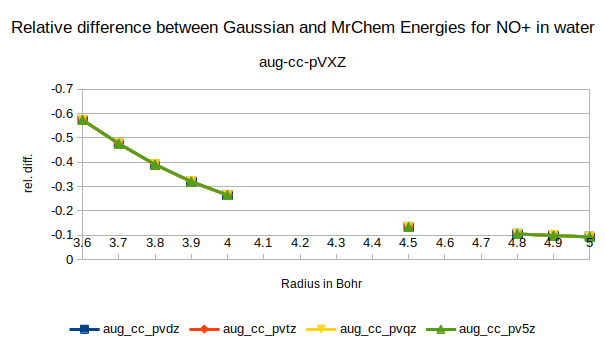
\includegraphics[width=\linewidth]{img/nopreldiff.png}
  \end{subfigure}
  \begin{subfigure}[b]{\linewidth}
    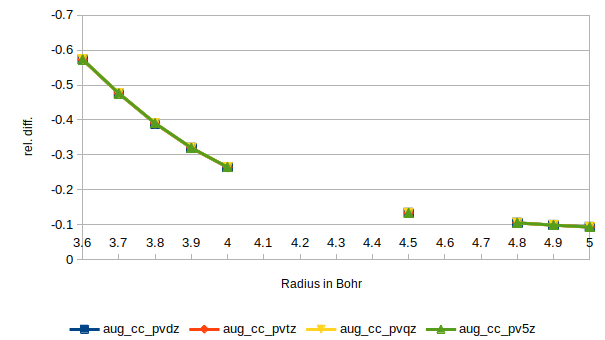
\includegraphics[width=\linewidth]{img/nopaugreldiff.png}
  \end{subfigure}
  \begin{subfigure}[b]{\linewidth}
    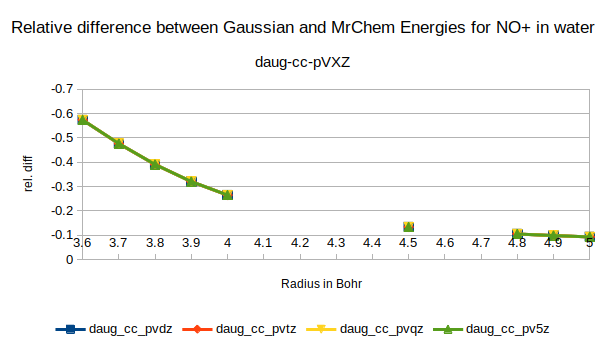
\includegraphics[width=\linewidth]{img/nopdaugreldiff.png}
  \end{subfigure}
  \caption{Relative difference between the Reaction field energy of \ce{NO^+} in a water solution calculated with MrChem
  and with different basis sets in Gaussian}
  \label{fig:nopreldiff}
\end{figure}

\begin{figure}[h!]
  \centering
  \begin{subfigure}[b]{\linewidth}
    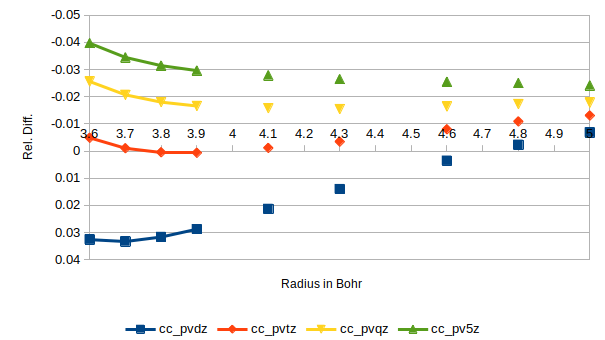
\includegraphics[width=\linewidth]{img/cyanreldiff.png}
  \end{subfigure}
  \begin{subfigure}[b]{\linewidth}
    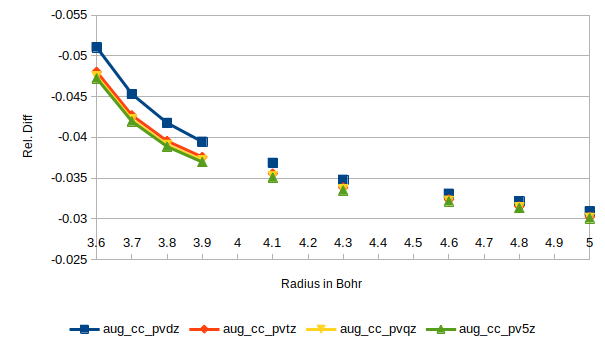
\includegraphics[width=\linewidth]{img/cyanaugreldiff.png}
  \end{subfigure}
  \begin{subfigure}[b]{\linewidth}
    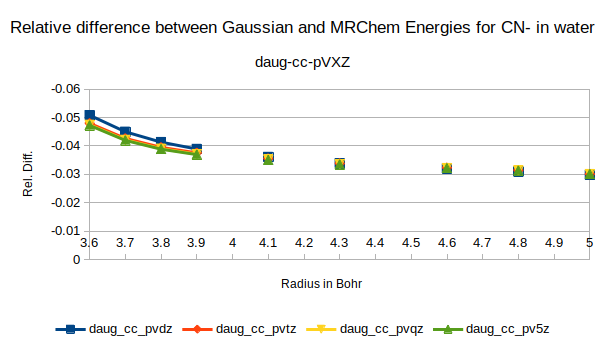
\includegraphics[width=\linewidth]{img/cyandaugreldiff.png}
  \end{subfigure}
  \caption{Relative difference between the Reaction field energy of \ce{CN^-} in a water solution calculated with MrChem
  and with different basis sets in Gaussian}
  \label{fig:cyanreldiff}
\end{figure}


We have observed that when, in Mrchem,  using a slightly bigger cavity than
Gaussian would give us a better difference between the Mrchem and Gaussian values.
In the following figures %\ref{fig:watreldiff02} \ref{fig:nopreldiff02} \ref{fig:cyanreldiff02}
we compared a calculation in gaussian with a given radius $r$
against an Mrchem calculation with radius $r + 0.2$Bohr for all the tests



We ran \ac{ABC} calcualtions in the same manner as above, here are the results for
each of the substrates in tables %numerate them
As we did above we increased the radius with $0.2$ Bohr in the hopes to see a
better correspondence


\subsection{Chipman Comparison}
In this part of the tests we simply compared our calculations to Chipman \cite{Chipman2002}.
They ran several calculations using different \ac{PCM} models, some of which were
explained in section \ref{approchessolv}. Here we will simply present our results
compared to theirs.


\section{Discussion}
\section{Conclusion}
\section{Areas of improvement/future development}

\section{Data tables}\label{Datatables}
\begin{sidewaystable}[h]

  \ttabbox{
  \resizebox{\textwidth}{!}{
  \begin{tabular}{|l|r|r|r|r|r|r|r|r|r|r|r|r|r|r|r|r|}
    \hline
    basis & \multicolumn{1}{l|}{vacuum E} & 3.6 & 3.7 & 3.8 & 3.9 & 4 & 4.1 & 4.2 & 4.3 & 4.4 & 4.5 & 4.6 & 4.7 & 4.8 & 4.9 & 5 \\ \hline
    Cc-pVDZ & -7.6027E+01 & -7.6039E+01 & -7.6038E+01 & -7.6036E+01 & -7.6035E+01 & -7.6035E+01 & -7.6034E+01 & -7.6033E+01 & -7.6033E+01 & -7.6032E+01 & -7.6032E+01 & -7.6031E+01 & -7.6031E+01 & -7.6031E+01 & -7.6030E+01 & -7.6030E+01 \\ \hline
    Cc-pVTZ & -7.6057E+01 & -7.6070E+01 & -7.6069E+01 & -7.6067E+01 & -7.6066E+01 & -7.6065E+01 & -7.6064E+01 & -7.6064E+01 & -7.6063E+01 & -7.6063E+01 & -7.6062E+01 & -7.6062E+01 & -7.6061E+01 & -7.6061E+01 & -7.6061E+01 & -7.6060E+01  \\ \hline
    Cc-pVQZ & -7.6065E+01 & -7.6078E+01 & -7.6076E+01 & -7.6075E+01 & -7.6074E+01 & -7.6073E+01 & -7.6072E+01 & -7.6071E+01 & -7.6071E+01 & -7.6070E+01 & -7.6070E+01 & -7.6069E+01 & -7.6069E+01 & -7.6069E+01 & -7.6068E+01 & -7.6068E+01  \\ \hline
    Cc-pV5Z & -7.6067E+01 & -7.6080E+01 & -7.6079E+01 & -7.6077E+01 & -7.6076E+01 & -7.6075E+01 & -7.6074E+01 & -7.6074E+01 & -7.6073E+01 & -7.6073E+01 & -7.6072E+01 & -7.6072E+01 & -7.6071E+01 & -7.6071E+01 & -7.6071E+01 & -7.6070E+01  \\ \hline
    Aug-cc-pVDZ & -7.6041E+01 & -7.6054E+01 & -7.6053E+01 & -7.6052E+01 & -7.6050E+01 & -7.6050E+01 & -7.6049E+01 & -7.6048E+01 & -7.6047E+01 & -7.6047E+01 & -7.6046E+01 & -7.6046E+01 & -7.6046E+01 & -7.6045E+01 & -7.6045E+01 & -7.6045E+01  \\ \hline
    Aug-cc-pVTZ & -7.6060E+01 & -7.6074E+01 & -7.6072E+01 & -7.6071E+01 & -7.6070E+01 & -7.6069E+01 & -7.6068E+01 & -7.6067E+01 & -7.6067E+01 & -7.6066E+01 & -7.6066E+01 & -7.6065E+01 & -7.6065E+01 & -7.6064E+01 & -7.6064E+01 & -7.6064E+01  \\ \hline
    Aug-cc-pVQZ & -7.6066E+01 & -7.6079E+01 & -7.6077E+01 & -7.6076E+01 & -7.6075E+01 & -7.6074E+01 & -7.6073E+01 & -7.6073E+01 & -7.6072E+01 & -7.6071E+01 & -7.6071E+01 & -7.6070E+01 & -7.6070E+01 & -7.6070E+01 & -7.6069E+01 & -7.6069E+01  \\ \hline
    Aug-cc-pV5Z & -7.6067E+01 & -7.6080E+01 & -7.6079E+01 & -7.6077E+01 & -7.6076E+01 & -7.6075E+01 & -7.6075E+01 & -7.6074E+01 & -7.6073E+01 & -7.6073E+01 & -7.6072E+01 & -7.6072E+01 & -7.6071E+01 & -7.6071E+01 & -7.6071E+01 & -7.6071E+01  \\ \hline
    daug-cc-pVDZ & -7.6042E+01 & -7.6055E+01 & -7.6053E+01 & -7.6052E+01 & -7.6051E+01 & -7.6050E+01 & -7.6049E+01 & -7.6049E+01 & -7.6048E+01 & -7.6047E+01 & -7.6047E+01 & -7.6046E+01 & -7.6046E+01 & -7.6046E+01 & -7.6045E+01 & -7.6045E+01  \\ \hline
    daug-cc-pVTZ & -7.6061E+01 & -7.6074E+01 & -7.6072E+01 & -7.6071E+01 & -7.6070E+01 & -7.6069E+01 & -7.6068E+01 & -7.6067E+01 & -7.6067E+01 & -7.6066E+01 & -7.6066E+01 & -7.6065E+01 & -7.6065E+01 & -7.6064E+01 & -7.6064E+01 & -7.6064E+01  \\ \hline
    daug-cc-pVQZ & -7.6066E+01 & -7.6079E+01 & -7.6077E+01 & -7.6076E+01 & -7.6075E+01 & -7.6074E+01 & -7.6073E+01 & -7.6073E+01 & -7.6072E+01 & -7.6071E+01 & -7.6071E+01 & -7.6071E+01 & -7.6070E+01 & -7.6070E+01 & -7.6069E+01 & -7.6069E+01 \\ \hline
    daug-cc-pV5Z & -7.6067E+01 & -7.6080E+01 & -7.6079E+01 & -7.6077E+01 & -7.6076E+01 & -7.6075E+01 & -7.6075E+01 & -7.6074E+01 & -7.6073E+01 & -7.6073E+01 & -7.6072E+01 & -7.6072E+01 & -7.6071E+01 & -7.6071E+01 & -7.6071E+01 & -7.6071E+01 \\ \hline
    mrchem & -7.6067E+01 & -7.6085E+01 & -7.6083E+01 & -7.6081E+01 & -7.6079E+01 & -7.6078E+01 & -7.6076E+01 & -7.6075E+01 & -7.6075E+01 & -7.6074E+01 & -7.6073E+01 & -7.6073E+01 & -7.6072E+01 & -7.6072E+01 & -7.6071E+01 & -7.4670E+01  \\ \hline
    variational & -7.6067E+01 & -7.6247E+01 & -7.6160E+01 & -7.6090E+01 & -7.6034E+01 & -7.5989E+01 & -7.5955E+01 & -7.5928E+01 & -7.5908E+01 & -7.5894E+01 & -7.5884E+01 & -7.5878E+01 & -7.5875E+01 & -7.5874E+01 & -7.5875E+01 & -7.4566E+01  \\ \hline
  \end{tabular}}}{\caption{Total Energy of \ce{H_2O}. Radius in top row in Bohr and energies in Hartree}
  \label{tab:rawwatdata}}

\ttabbox{

  \resizebox{\textwidth}{!}{
  \begin{tabular}{|l|r|r|r|r|r|r|r|r|r|r|r|r|r|r|r|r|}
    \hline
    basis & \multicolumn{1}{l|}{vac} & 3.6 & 3.7 & 3.8 & 3.9 & 4 & 4.1 & 4.2 & 4.3 & 4.4 & 4.5 & 4.6 & 4.7 & 4.8 & 4.9 & 5 \\ \hline
    Cc-pVDZ & -1.2893E+02 & -1.2907E+02 & -1.2906E+02 & -1.2906E+02 & -1.2906E+02 & -1.2905E+02 & -1.2905E+02 & -1.2905E+02 & -1.2904E+02 & -1.2904E+02 & -1.2904E+02 & -1.2904E+02 & -1.2903E+02 & -1.2903E+02 & -1.2903E+02 & -1.2903E+02 \\ \hline
    Cc-pVTZ & -1.2897E+02 & -1.2911E+02 & -1.2910E+02 & -1.2910E+02 & -1.2910E+02 & -1.2909E+02 & -1.2909E+02 & -1.2909E+02 & -1.2908E+02 & -1.2908E+02 & -1.2908E+02 & -1.2907E+02 & -1.2907E+02 & -1.2907E+02 & -1.2907E+02 & -1.2907E+02 \\ \hline
    Cc-pVQZ & -1.2898E+02 & -1.2912E+02 & -1.2911E+02 & -1.2911E+02 & -1.2911E+02 & -1.2910E+02 & -1.2910E+02 & -1.2910E+02 & -1.2909E+02 & -1.2909E+02 & -1.2909E+02 & -1.2908E+02 & -1.2908E+02 & -1.2908E+02 & -1.2908E+02 & -1.2908E+02 \\ \hline
    Cc-pV5Z & -1.2898E+02 & -1.2912E+02 & -1.2912E+02 & -1.2911E+02 & -1.2911E+02 & -1.2910E+02 & -1.2910E+02 & -1.2910E+02 & -1.2909E+02 & -1.2909E+02 & -1.2909E+02 & -1.2909E+02 & -1.2908E+02 & -1.2908E+02 & -1.2908E+02 & -1.2908E+02 \\ \hline
    Aug-cc-pVDZ & -1.2894E+02 & -1.2908E+02 & -1.2907E+02 & -1.2907E+02 & -1.2906E+02 & -1.2906E+02 & -1.2906E+02 & -1.2905E+02 & -1.2905E+02 & -1.2905E+02 & -1.2905E+02 & -1.2904E+02 & -1.2904E+02 & -1.2904E+02 & -1.2904E+02 & -1.2903E+02 \\ \hline
    Aug-cc-pVTZ & -1.2897E+02 & -1.2911E+02 & -1.2910E+02 & -1.2910E+02 & -1.2910E+02 & -1.2909E+02 & -1.2909E+02 & -1.2909E+02 & -1.2908E+02 & -1.2908E+02 & -1.2908E+02 & -1.2908E+02 & -1.2907E+02 & -1.2907E+02 & -1.2907E+02 & -1.2907E+02 \\ \hline
    Aug-cc-pVQZ & -1.2898E+02 & -1.2912E+02 & -1.2911E+02 & -1.2911E+02 & -1.2911E+02 & -1.2910E+02 & -1.2910E+02 & -1.2910E+02 & -1.2909E+02 & -1.2909E+02 & -1.2909E+02 & -1.2909E+02 & -1.2908E+02 & -1.2908E+02 & -1.2908E+02 & -1.2908E+02 \\ \hline
    Aug-cc-pV5Z & -1.2898E+02 & -1.2912E+02 & -1.2912E+02 & -1.2911E+02 & -1.2911E+02 & -1.2910E+02 & -1.2910E+02 & -1.2910E+02 & -1.2909E+02 & -1.2909E+02 & -1.2909E+02 & -1.2909E+02 & -1.2908E+02 & -1.2908E+02 & -1.2908E+02 & -1.2908E+02 \\ \hline
    daug-cc-pVDZ & -1.2894E+02 & -1.2908E+02 & -1.2907E+02 & -1.2907E+02 & -1.2906E+02 & -1.2906E+02 & -1.2906E+02 & -1.2905E+02 & -1.2905E+02 & -1.2905E+02 & -1.2905E+02 & -1.2904E+02 & -1.2904E+02 & -1.2904E+02 & -1.2904E+02 & -1.2904E+02 \\ \hline
    daug-cc-pVTZ & -1.2897E+02 & -1.2911E+02 & -1.2910E+02 & -1.2910E+02 & -1.2910E+02 & -1.2909E+02 & -1.2909E+02 & -1.2909E+02 & -1.2908E+02 & -1.2908E+02 & -1.2908E+02 & -1.2908E+02 & -1.2907E+02 & -1.2907E+02 & -1.2907E+02 & -1.2907E+02 \\ \hline
    daug-cc-pVQZ & -1.2898E+02 & -1.2912E+02 & -1.2911E+02 & -1.2911E+02 & -1.2911E+02 & -1.2910E+02 & -1.2910E+02 & -1.2910E+02 & -1.2909E+02 & -1.2909E+02 & -1.2909E+02 & -1.2909E+02 & -1.2908E+02 & -1.2908E+02 & -1.2908E+02 & -1.2908E+02 \\ \hline
    daug-cc-pV5Z & -1.2898E+02 & -1.2912E+02 & -1.2912E+02 & -1.2911E+02 & -1.2911E+02 & -1.2910E+02 & -1.2910E+02 & -1.2910E+02 & -1.2909E+02 & -1.2909E+02 & -1.2909E+02 & -1.2909E+02 & -1.2908E+02 & -1.2908E+02 & -1.2908E+02 & -1.2908E+02 \\ \hline
    mrchem & -1.2898E+02 & -1.2931E+02 & -1.2924E+02 & -1.2920E+02 & -1.2917E+02 & -1.2915E+02 & -1.2566E+02 & \multicolumn{1}{l|}{N/A} & -1.2565E+02 & -1.2565E+02 & -1.2911E+02 & \multicolumn{1}{l|}{N/A} & -1.2564E+02 & -1.2909E+02 & -1.2909E+02 & -1.2909E+02 \\ \hline
    variational & -1.2898E+02 & -1.2794E+02 & -1.2781E+02 & -1.2789E+02 & -1.2808E+02 & -1.2830E+02 & -1.2566E+02 & \multicolumn{1}{l|}{N/A} & -1.2565E+02 & -1.2565E+02 & -1.2900E+02 & -1.2905E+02 & -1.2564E+02 & -1.2909E+02 & -1.2910E+02 & -1.2910E+02 \\ \hline
  \end{tabular}}}{\caption{Total Energy of \ce{NO^+}.  Radius in top row in Bohr and energies in Hartree}
  \label{tab:rawnopdata}}


\ttabbox{

\resizebox{\textwidth}{!}{
\begin{tabular}{|l|r|r|r|r|r|r|r|r|r|r|r|r|r|r|r|r|}
\hline
basis & \multicolumn{1}{l|}{vac} & 3.6 & 3.7 & 3.8 & 3.9 & 4 & 4.1 & 4.2 & 4.3 & 4.4 & 4.5 & 4.6 & 4.7 & 4.8 & 4.9 & 5 \\ \hline
Cc-pVDZ & -7.6027E+01 & -9.2425E+01 & -9.2425E+01 & -9.2423E+01 & -9.2422E+01 & -9.2420E+01 & -9.2418E+01 & -9.2416E+01 & -9.2414E+01 & -9.2412E+01 & -9.2410E+01 & -9.2408E+01 & -9.2405E+01 & -9.2403E+01 & -9.2401E+01 & -9.2399E+01  \\ \hline
Cc-pVTZ & -7.6057E+01 & -9.2455E+01 & -9.2455E+01 & -9.2454E+01 & -9.2453E+01 & -9.2452E+01 & -9.2451E+01 & -9.2449E+01 & -9.2447E+01 & -9.2445E+01 & -9.2443E+01 & -9.2441E+01 & -9.2439E+01 & -9.2437E+01 & -9.2435E+01 & -9.2433E+01  \\ \hline
Cc-pVQZ & -7.6065E+01 & -9.2464E+01 & -9.2463E+01 & -9.2463E+01 & -9.2462E+01 & -9.2461E+01 & -9.2460E+01 & -9.2458E+01 & -9.2456E+01 & -9.2455E+01 & -9.2453E+01 & -9.2451E+01 & -9.2449E+01 & -9.2447E+01 & -9.2445E+01 & -9.2443E+01  \\ \hline
Cc-pV5Z & -7.6067E+01 & -9.2465E+01 & -9.2465E+01 & -9.2465E+01 & -9.2464E+01 & -9.2463E+01 & -9.2462E+01 & -9.2460E+01 & -9.2459E+01 & -9.2457E+01 & -9.2455E+01 & -9.2454E+01 & -9.2452E+01 & -9.2450E+01 & -9.2448E+01 & -9.2446E+01  \\ \hline
Aug-cc-pVDZ & -7.6041E+01 & -9.2441E+01 & -9.2441E+01 & -9.2440E+01 & -9.2439E+01 & -9.2438E+01 & -9.2437E+01 & -9.2436E+01 & -9.2434E+01 & -9.2433E+01 & -9.2431E+01 & -9.2429E+01 & -9.2427E+01 & -9.2426E+01 & -9.2424E+01 & -9.2422E+01  \\ \hline
Aug-cc-pVTZ & -7.6060E+01 & -9.2459E+01 & -9.2459E+01 & -9.2459E+01 & -9.2458E+01 & -9.2457E+01 & -9.2456E+01 & -9.2454E+01 & -9.2453E+01 & -9.2451E+01 & -9.2449E+01 & -9.2448E+01 & -9.2446E+01 & -9.2444E+01 & -9.2442E+01 & -9.2441E+01  \\ \hline
Aug-cc-pVQZ & -7.6066E+01 & -9.2465E+01 & -9.2465E+01 & -9.2464E+01 & -9.2463E+01 & -9.2462E+01 & -9.2461E+01 & -9.2460E+01 & -9.2458E+01 & -9.2456E+01 & -9.2455E+01 & -9.2453E+01 & -9.2451E+01 & -9.2449E+01 & -9.2448E+01 & -9.2446E+01  \\ \hline
Aug-cc-pV5Z & -7.6067E+01 & -9.2466E+01 & -9.2466E+01 & -9.2465E+01 & -9.2464E+01 & -9.2463E+01 & -9.2462E+01 & -9.2461E+01 & -9.2459E+01 & -9.2457E+01 & -9.2456E+01 & -9.2454E+01 & -9.2452E+01 & -9.2450E+01 & -9.2449E+01 & -9.2447E+01  \\ \hline
daug-cc-pVDZ & -7.6042E+01 & -9.2441E+01 & -9.2441E+01 & -9.2440E+01 & -9.2440E+01 & -9.2439E+01 & -9.2437E+01 & -9.2436E+01 & -9.2435E+01 & -9.2433E+01 & -9.2431E+01 & -9.2430E+01 & -9.2428E+01 & -9.2426E+01 & -9.2424E+01 & -9.2423E+01  \\ \hline
daug-cc-pVTZ & -7.6061E+01 & -9.2459E+01 & -9.2459E+01 & -9.2459E+01 & -9.2458E+01 & -9.2457E+01 & -9.2456E+01 & -9.2454E+01 & -9.2453E+01 & -9.2451E+01 & -9.2449E+01 & -9.2448E+01 & -9.2446E+01 & -9.2444E+01 & -9.2443E+01 & -9.2441E+01  \\ \hline
daug-cc-pVQZ & -7.6066E+01 & -9.2465E+01 & -9.2465E+01 & -9.2464E+01 & -9.2463E+01 & -9.2462E+01 & -9.2461E+01 & -9.2460E+01 & -9.2458E+01 & -9.2456E+01 & -9.2455E+01 & -9.2453E+01 & -9.2451E+01 & -9.2449E+01 & -9.2448E+01 & -9.2446E+01  \\ \hline
daug-cc-pV5Z & -7.6067E+01 & -9.2466E+01 & -9.2466E+01 & -9.2465E+01 & -9.2464E+01 & -9.2463E+01 & -9.2462E+01 & -9.2461E+01 & -9.2459E+01 & -9.2457E+01 & -9.2456E+01 & -9.2454E+01 & -9.2452E+01 & -9.2450E+01 & -9.2449E+01 & -9.2447E+01  \\ \hline
mrchem & -9.2349E+01 & -9.2472E+01 & -9.2471E+01 & -9.2470E+01 & -9.2469E+01 & -8.9965E+01 & -9.2466E+01 & \multicolumn{1}{l|}{N/A} & -9.2463E+01 & \multicolumn{1}{l|}{N/A} & -8.9954E+01 & -9.2458E+01 & \multicolumn{1}{l|}{N/A} & -9.2454E+01 & -8.9945E+01 & -9.2450E+01  \\ \hline
variational & -9.2349E+01 & -9.7694E+01 & -9.7347E+01 & -9.6991E+01 & -9.6630E+01 & -9.6271E+01 & -9.5920E+01 & \multicolumn{1}{l|}{N/A} & -9.5263E+01 & \multicolumn{1}{l|}{N/A} & -9.4678E+01 & -9.4432E+01 & -9.4199E+01 & -9.3990E+01 & -9.3801E+01 & -9.3632E+01  \\ \hline
\end{tabular}}} {\caption{Total Energy of \ce{CN^-}.  Radius in top row in Bohr and energies in Hartree}
\label{tab:rawcyandata}}

\ttabbox{

\resizebox{\textwidth}{!}{

\begin{tabular}{|l|r|r|r|r|r|r|r|r|r|r|r|r|r|r|r|r|}
\hline
basis & \multicolumn{1}{l|}{vac} & 3.6 & 3.7 & 3.8 & 3.9 & 4 & 4.1 & 4.2 & 4.3 & 4.4 & 4.5 & 4.6 & 4.7 & 4.8 & 4.9 & 5 \\ \hline
Cc-pVDZ & -7.2361E+00 & -7.3732E+00 & -7.3695E+00 & -7.3660E+00 & -7.3627E+00 & -7.3595E+00 & -7.3565E+00 & -7.3536E+00 & -7.3509E+00 & -7.3483E+00 & -7.3458E+00 & -7.3434E+00 & -7.3411E+00 & -7.3390E+00 & -7.3369E+00 & -7.3348E+00 \\ \hline
Cc-pVTZ & -7.2364E+00 & -7.3735E+00 & -7.3698E+00 & -7.3663E+00 & -7.3629E+00 & -7.3598E+00 & -7.3568E+00 & -7.3539E+00 & -7.3512E+00 & -7.3486E+00 & -7.3461E+00 & -7.3437E+00 & -7.3414E+00 & -7.3392E+00 & -7.3371E+00 & -7.3351E+00 \\ \hline
Cc-pVQZ & -7.2364E+00 & -7.3735E+00 & -7.3698E+00 & -7.3663E+00 & -7.3630E+00 & -7.3598E+00 & -7.3568E+00 & -7.3539E+00 & -7.3512E+00 & -7.3486E+00 & -7.3461E+00 & -7.3437E+00 & -7.3414E+00 & -7.3392E+00 & -7.3371E+00 & -7.3351E+00 \\ \hline
Cc-pV5Z & -7.2364E+00 & -7.3735E+00 & -7.3698E+00 & -7.3663E+00 & -7.3630E+00 & -7.3598E+00 & -7.3568E+00 & -7.3539E+00 & -7.3512E+00 & -7.3486E+00 & -7.3461E+00 & -7.3437E+00 & -7.3414E+00 & -7.3392E+00 & -7.3371E+00 & -7.3351E+00 \\ \hline
Aug-cc-pVDZ & -7.2361E+00 & -7.3732E+00 & -7.3695E+00 & -7.3660E+00 & -7.3627E+00 & -7.3595E+00 & -7.3565E+00 & -7.3536E+00 & -7.3509E+00 & -7.3483E+00 & -7.3458E+00 & -7.3434E+00 & -7.3411E+00 & -7.3390E+00 & -7.3369E+00 & -7.3348E+00 \\ \hline
Aug-cc-pVTZ & -7.2364E+00 & -7.3735E+00 & -7.3698E+00 & -7.3663E+00 & -7.3629E+00 & -7.3598E+00 & -7.3568E+00 & -7.3539E+00 & -7.3512E+00 & -7.3486E+00 & -7.3461E+00 & -7.3437E+00 & -7.3414E+00 & -7.3392E+00 & -7.3371E+00 & -7.3351E+00 \\ \hline
Aug-cc-pVQZ & -7.2364E+00 & -7.3735E+00 & -7.3698E+00 & -7.3663E+00 & -7.3630E+00 & -7.3598E+00 & -7.3568E+00 & -7.3539E+00 & -7.3512E+00 & -7.3486E+00 & -7.3461E+00 & -7.3437E+00 & -7.3414E+00 & -7.3392E+00 & -7.3371E+00 & -7.3351E+00 \\ \hline
Aug-cc-pV5Z & -7.2364E+00 & -7.3735E+00 & -7.3698E+00 & -7.3663E+00 & -7.3630E+00 & -7.3598E+00 & -7.3568E+00 & -7.3539E+00 & -7.3512E+00 & -7.3486E+00 & -7.3461E+00 & -7.3437E+00 & -7.3414E+00 & -7.3392E+00 & -7.3371E+00 & -7.3351E+00 \\ \hline
daug-cc-pVDZ & -7.2361E+00 & -7.3732E+00 & -7.3695E+00 & -7.3660E+00 & -7.3627E+00 & -7.3595E+00 & -7.3565E+00 & -7.3536E+00 & -7.3509E+00 & -7.3483E+00 & -7.3458E+00 & -7.3434E+00 & -7.3411E+00 & -7.3390E+00 & -7.3369E+00 & -7.3348E+00 \\ \hline
daug-cc-pVTZ & -7.2364E+00 & -7.3735E+00 & -7.3698E+00 & -7.3663E+00 & -7.3629E+00 & -7.3598E+00 & -7.3568E+00 & -7.3539E+00 & -7.3512E+00 & -7.3486E+00 & -7.3461E+00 & -7.3437E+00 & -7.3414E+00 & -7.3392E+00 & -7.3371E+00 & -7.3351E+00 \\ \hline
daug-cc-pVQZ & -7.2364E+00 & -7.3735E+00 & -7.3698E+00 & -7.3663E+00 & -7.3630E+00 & -7.3598E+00 & -7.3568E+00 & -7.3539E+00 & -7.3512E+00 & -7.3486E+00 & -7.3461E+00 & -7.3437E+00 & -7.3414E+00 & -7.3392E+00 & -7.3371E+00 & -7.3351E+00 \\ \hline
daug-cc-pV5Z & -7.2364E+00 & -7.3735E+00 & -7.3698E+00 & -7.3663E+00 & -7.3630E+00 & -7.3598E+00 & -7.3568E+00 & -7.3539E+00 & -7.3512E+00 & -7.3486E+00 & -7.3461E+00 & -7.3437E+00 & -7.3414E+00 & -7.3392E+00 & -7.3371E+00 & -7.3351E+00 \\ \hline
mrchem & -7.2364E+00 & -7.3792E+00 & -7.3752E+00 & -7.3714E+00 & -7.3678E+00 & -7.3644E+00 & -7.3612E+00 & -7.3581E+00 & -7.3551E+00 & -7.3524E+00 & -7.3497E+00 & -7.3472E+00 & -7.3447E+00 & -7.3424E+00 & -7.3402E+00 & -7.3380E+00 \\ \hline
variational & -7.2364E+00 & -7.3744E+00 & -7.3707E+00 & -7.3671E+00 & -7.3636E+00 & -7.3603E+00 & -7.3572E+00 & -7.3542E+00 & -7.3514E+00 & -7.3487E+00 & -7.3461E+00 & -7.3438E+00 & -7.3415E+00 & -7.3393E+00 & -7.3372E+00 & -7.3352E+00 \\ \hline
\end{tabular}}}{\caption{Total energy of \ce{Li^+}. Radius on top row in Bohr and energies in Hartree}
\label{tab:rawLipdata}}

\end{sidewaystable}

\begin{sidewaystable}
  \ttabbox{
  \resizebox{\textwidth}{!}{
    \begin{tabular}{|l|r|r|r|r|r|r|r|r|r|r|r|r|r|r|r|}
    \hline
    basis & 3.6 & 3.7 & 3.8 & 3.9 & 4 & 4.1 & 4.2 & 4.3 & 4.4 & 4.5 & 4.6 & 4.7 & 4.8 & 4.9 & 5 \\ \hline
    Cc-pVDZ & -1.2450E-02 & -1.0998E-02 & -9.7804E-03 & -8.7499E-03 & -7.8700E-03 & -7.1128E-03 & -6.4573E-03 & -5.8844E-03 & -5.3816E-03 & -4.9378E-03 & -4.5442E-03 & -4.1936E-03 & -3.8799E-03 & -3.5983E-03 & -3.3447E-03 \\ \hline
    Cc-pVTZ & -1.3097E-02 & -1.1545E-02 & -1.0243E-02 & -9.1412E-03 & -8.2007E-03 & -7.3922E-03 & -6.6939E-03 & -6.0843E-03 & -5.5504E-03 & -5.0804E-03 & -4.6646E-03 & -4.2951E-03 & -3.9654E-03 & -3.6700E-03 & -3.4049E-03 \\ \hline
    Cc-pVQZ & -1.3218E-02 & -1.1651E-02 & -1.0334E-02 & -9.2192E-03 & -8.2670E-03 & -7.4482E-03 & -6.7410E-03 & -6.1235E-03 & -5.5827E-03 & -5.1067E-03 & -4.6857E-03 & -4.3118E-03 & -3.9782E-03 & -3.6796E-03 & -3.4117E-03 \\ \hline
    Cc-pV5Z & -1.3284E-02 & -1.1713E-02 & -1.0393E-02 & -9.2737E-03 & -8.3174E-03 & -7.4945E-03 & -6.7834E-03 & -6.1620E-03 & -5.6175E-03 & -5.1380E-03 & -4.7138E-03 & -4.3369E-03 & -4.0007E-03 & -3.6996E-03 & -3.4295E-03 \\ \hline
    Aug-cc-pVDZ & -1.3190E-02 & -1.1634E-02 & -1.0328E-02 & -9.2204E-03 & -8.2741E-03 & -7.4596E-03 & -6.7553E-03 & -6.1396E-03 & -5.5997E-03 & -5.1238E-03 & -4.7025E-03 & -4.3279E-03 & -3.9935E-03 & -3.6939E-03 & -3.4249E-03 \\ \hline
    Aug-cc-pVTZ & -1.3238E-02 & -1.1670E-02 & -1.0353E-02 & -9.2358E-03 & -8.2817E-03 & -7.4605E-03 & -6.7510E-03 & -6.1309E-03 & -5.5876E-03 & -5.1091E-03 & -4.6858E-03 & -4.3097E-03 & -3.9742E-03 & -3.6739E-03 & -3.4045E-03 \\ \hline
    Aug-cc-pVQZ & -1.3221E-02 & -1.1655E-02 & -1.0338E-02 & -9.2227E-03 & -8.2695E-03 & -7.4493E-03 & -6.7407E-03 & -6.1214E-03 & -5.5789E-03 & -5.1011E-03 & -4.6784E-03 & -4.3029E-03 & -3.9680E-03 & -3.6681E-03 & -3.3992E-03 \\ \hline
    Aug-cc-pV5Z & -1.3223E-02 & -1.1655E-02 & -1.0337E-02 & -9.2207E-03 & -8.2672E-03 & -7.4469E-03 & -6.7383E-03 & -6.1192E-03 & -5.5769E-03 & -5.0994E-03 & -4.6770E-03 & -4.3018E-03 & -3.9672E-03 & -3.6676E-03 & -3.3988E-03 \\ \hline
    daug-cc-pVDZ & -1.3228E-02 & -1.1665E-02 & -1.0351E-02 & -9.2383E-03 & -8.2871E-03 & -7.4682E-03 & -6.7605E-03 & -6.1417E-03 & -5.5992E-03 & -5.1213E-03 & -4.6983E-03 & -4.3223E-03 & -3.9868E-03 & -3.6863E-03 & -3.4166E-03 \\ \hline
    daug-cc-pVTZ & -1.3243E-02 & -1.1675E-02 & -1.0357E-02 & -9.2398E-03 & -8.2849E-03 & -7.4631E-03 & -6.7529E-03 & -6.1322E-03 & -5.5882E-03 & -5.1092E-03 & -4.6855E-03 & -4.3091E-03 & -3.9734E-03 & -3.6729E-03 & -3.4034E-03 \\ \hline
    daug-cc-pVQZ & -1.3223E-02 & -1.1656E-02 & -1.0340E-02 & -9.2243E-03 & -8.2711E-03 & -7.4508E-03 & -6.7421E-03 & -6.1227E-03 & -5.5800E-03 & -5.1021E-03 & -4.6793E-03 & -4.3037E-03 & -3.9686E-03 & -3.6687E-03 & -3.3997E-03 \\ \hline
    daug-cc-pV5Z & -1.3224E-02 & -1.1655E-02 & -1.0337E-02 & -9.2210E-03 & -8.2674E-03 & -7.4470E-03 & -6.7385E-03 & -6.1193E-03 & -5.5770E-03 & -5.0995E-03 & -4.6771E-03 & -4.3019E-03 & -3.9672E-03 & -3.6676E-03 & -3.3988E-03 \\ \hline
    mrchem & -1.8036E-02 & -1.5494E-02 & -1.3437E-02 & -1.1751E-02 & -1.0354E-02 & -9.1865E-03 & -8.1992E-03 & -7.3577E-03 & -6.6339E-03 & -6.0092E-03 & -5.4647E-03 & -4.9879E-03 & -4.5682E-03 & -4.1968E-03 & 1.3975E+00 \\ \hline
    variational & -1.7939E-01 & -9.2889E-02 & -2.2807E-02 & 3.3437E-02 & 7.7993E-02 & 1.1246E-01 & 1.3945E-01 & 1.5927E-01 & 1.7367E-01 & 1.8347E-01 & 1.8957E-01 & 1.9266E-01 & 1.9338E-01 & 1.9217E-01 & 1.5012E+00 \\ \hline
    \end{tabular}}}{  \caption{Reaction field energy of \ce{H_2O}. Radius on top row in Bohr and energies in Hartree}\label{tab:Erdatawat}}

  \ttabbox{
  \resizebox{\textwidth}{!}{
  \begin{tabular}{|l|r|r|r|r|r|r|r|r|r|r|r|r|r|r|r|r|r|}
  \hline
  basis & 3.6 & 3.7 & 3.8 & 3.9 & 4 & 4.1 & 4.2 & 4.3 & 4.4 & 4.5 & 4.6 & 4.7 & 4.8 & 4.9 & 5 & \multicolumn{1}{l|}{} & \multicolumn{1}{l|}{} \\ \hline
  Cc-pVDZ & -1.4058E-01 & -1.3613E-01 & -1.3206E-01 & -1.2830E-01 & -1.2481E-01 & -1.2155E-01 & -1.1849E-01 & -1.1561E-01 & -1.1289E-01 & -1.1031E-01 & -1.0785E-01 & -1.0551E-01 & -1.0327E-01 & -1.0114E-01 & -9.9088E-02 & -1.2929E-01 & -1.2239E-01 \\ \hline
  Cc-pVTZ & -1.4064E-01 & -1.3621E-01 & -1.3214E-01 & -1.2839E-01 & -1.2489E-01 & -1.2162E-01 & -1.1854E-01 & -1.1565E-01 & -1.1291E-01 & -1.1032E-01 & -1.0785E-01 & -1.0550E-01 & -1.0326E-01 & -1.0112E-01 & -9.9067E-02 & -1.2916E-01 & -1.2227E-01 \\ \hline
  Cc-pVQZ & -1.4042E-01 & -1.3604E-01 & -1.3202E-01 & -1.2829E-01 & -1.2482E-01 & -1.2157E-01 & -1.1851E-01 & -1.1563E-01 & -1.1290E-01 & -1.1031E-01 & -1.0785E-01 & -1.0550E-01 & -1.0326E-01 & -1.0112E-01 & -9.9068E-02 & -1.2909E-01 & -1.2223E-01 \\ \hline
  Cc-pV5Z & -1.4032E-01 & -1.3595E-01 & -1.3193E-01 & -1.2821E-01 & -1.2475E-01 & -1.2151E-01 & -1.1846E-01 & -1.1559E-01 & -1.1287E-01 & -1.1028E-01 & -1.0783E-01 & -1.0549E-01 & -1.0325E-01 & -1.0111E-01 & -9.9059E-02 & -1.2900E-01 & -1.2218E-01 \\ \hline
  Aug-cc-pVDZ & -1.4051E-01 & -1.3606E-01 & -1.3200E-01 & -1.2824E-01 & -1.2476E-01 & -1.2150E-01 & -1.1844E-01 & -1.1556E-01 & -1.1284E-01 & -1.1026E-01 & -1.0780E-01 & -1.0546E-01 & -1.0323E-01 & -1.0109E-01 & -9.9045E-02 & -1.2887E-01 & -1.2206E-01 \\ \hline
  Aug-cc-pVTZ & -1.4048E-01 & -1.3608E-01 & -1.3203E-01 & -1.2829E-01 & -1.2481E-01 & -1.2156E-01 & -1.1849E-01 & -1.1561E-01 & -1.1288E-01 & -1.1029E-01 & -1.0783E-01 & -1.0549E-01 & -1.0325E-01 & -1.0111E-01 & -9.9056E-02 & -1.2902E-01 & -1.2216E-01 \\ \hline
  Aug-cc-pVQZ & -1.4036E-01 & -1.3598E-01 & -1.3196E-01 & -1.2824E-01 & -1.2478E-01 & -1.2153E-01 & -1.1848E-01 & -1.1560E-01 & -1.1288E-01 & -1.1029E-01 & -1.0783E-01 & -1.0549E-01 & -1.0325E-01 & -1.0111E-01 & -9.9059E-02 & -1.2903E-01 & -1.2218E-01 \\ \hline
  Aug-cc-pV5Z & -1.4032E-01 & -1.3594E-01 & -1.3193E-01 & -1.2821E-01 & -1.2475E-01 & -1.2151E-01 & -1.1846E-01 & -1.1558E-01 & -1.1286E-01 & -1.1028E-01 & -1.0783E-01 & -1.0548E-01 & -1.0325E-01 & -1.0111E-01 & -9.9058E-02 & -1.2900E-01 & -1.2217E-01 \\ \hline
  daug-cc-pVDZ & -1.4043E-01 & -1.3601E-01 & -1.3196E-01 & -1.2823E-01 & -1.2475E-01 & -1.2150E-01 & -1.1845E-01 & -1.1558E-01 & -1.1286E-01 & -1.1028E-01 & -1.0783E-01 & -1.0549E-01 & -1.0325E-01 & -1.0112E-01 & -9.9068E-02 & -1.2889E-01 & -1.2208E-01 \\ \hline
  daug-cc-pVTZ & -1.4040E-01 & -1.3601E-01 & -1.3198E-01 & -1.2825E-01 & -1.2478E-01 & -1.2153E-01 & -1.1847E-01 & -1.1560E-01 & -1.1287E-01 & -1.1029E-01 & -1.0783E-01 & -1.0549E-01 & -1.0325E-01 & -1.0111E-01 & -9.9059E-02 & -1.2900E-01 & -1.2216E-01 \\ \hline
  daug-cc-pVQZ & -1.4034E-01 & -1.3596E-01 & -1.3194E-01 & -1.2822E-01 & -1.2476E-01 & -1.2152E-01 & -1.1846E-01 & -1.1559E-01 & -1.1287E-01 & -1.1028E-01 & -1.0783E-01 & -1.0548E-01 & -1.0325E-01 & -1.0111E-01 & -9.9058E-02 & -1.2902E-01 & -1.2218E-01 \\ \hline
  daug-cc-pV5Z & -1.4032E-01 & -1.3594E-01 & -1.3193E-01 & -1.2821E-01 & -1.2475E-01 & -1.2151E-01 & -1.1846E-01 & -1.1558E-01 & -1.1286E-01 & -1.1028E-01 & -1.0782E-01 & -1.0548E-01 & -1.0325E-01 & -1.0111E-01 & -9.9058E-02 & -1.2900E-01 & -1.2217E-01 \\ \hline
  mrchem & -3.2883E-01 & -2.5954E-01 & -2.1649E-01 & -1.8860E-01 & -1.6969E-01 & 3.3235E+00 & N/A & 3.3308E+00 & 3.3341E+00 & -1.2727E-01 & N/A & 3.3429E+00 & -1.1538E-01 & -1.1218E-01 & -1.0924E-01 & -1.3411E-01 & -1.2670E-01 \\ \hline
  variational & 1.0359E+00 & 1.1729E+00 & 1.0849E+00 & 8.9494E-01 & 6.7670E-01 & 3.3235E+00 & N/A & 3.3308E+00 & 3.3341E+00 & -2.0407E-02 & -6.8498E-02 & 3.3429E+00 & -1.1235E-01 & -1.1730E-01 & -1.1578E-01 & -1.8326E-01 & -1.5337E-01 \\ \hline
  \end{tabular}}}{\caption{Reaction field energy of \ce{NO^+}. Radius on top row in Bohr and energies in Hartree}
  \label{tab:Erdatanop}}

  \ttabbox{
  \resizebox{\textwidth}{!}{
\begin{tabular}{|l|r|r|r|r|r|r|r|r|r|r|r|r|r|r|r|}
\hline
basis & 3.6 & 3.7 & 3.8 & 3.9 & 4 & 4.1 & 4.2 & 4.3 & 4.4 & 4.5 & 4.6 & 4.7 & 4.8 & 4.9 & 5 \\ \hline
Cc-pVDZ & -1.6399E+01 & -1.6398E+01 & -1.6397E+01 & -1.6395E+01 & -1.6394E+01 & -1.6392E+01 & -1.6390E+01 & -1.6388E+01 & -1.6385E+01 & -1.6383E+01 & -1.6381E+01 & -1.6379E+01 & -1.6377E+01 & -1.6374E+01 & -1.6372E+01 \\ \hline
Cc-pVTZ & -1.6398E+01 & -1.6398E+01 & -1.6398E+01 & -1.6396E+01 & -1.6395E+01 & -1.6394E+01 & -1.6392E+01 & -1.6390E+01 & -1.6388E+01 & -1.6386E+01 & -1.6384E+01 & -1.6382E+01 & -1.6380E+01 & -1.6378E+01 & -1.6376E+01 \\ \hline
Cc-pVQZ & -1.6399E+01 & -1.6399E+01 & -1.6398E+01 & -1.6397E+01 & -1.6396E+01 & -1.6395E+01 & -1.6393E+01 & -1.6392E+01 & -1.6390E+01 & -1.6388E+01 & -1.6386E+01 & -1.6384E+01 & -1.6383E+01 & -1.6381E+01 & -1.6379E+01 \\ \hline
Cc-pV5Z & -1.6399E+01 & -1.6399E+01 & -1.6398E+01 & -1.6397E+01 & -1.6396E+01 & -1.6395E+01 & -1.6393E+01 & -1.6392E+01 & -1.6390E+01 & -1.6388E+01 & -1.6387E+01 & -1.6385E+01 & -1.6383E+01 & -1.6381E+01 & -1.6380E+01 \\ \hline
Aug-cc-pVDZ & -1.6399E+01 & -1.6399E+01 & -1.6399E+01 & -1.6398E+01 & -1.6397E+01 & -1.6396E+01 & -1.6395E+01 & -1.6393E+01 & -1.6391E+01 & -1.6390E+01 & -1.6388E+01 & -1.6386E+01 & -1.6384E+01 & -1.6383E+01 & -1.6381E+01 \\ \hline
Aug-cc-pVTZ & -1.6399E+01 & -1.6399E+01 & -1.6398E+01 & -1.6398E+01 & -1.6396E+01 & -1.6395E+01 & -1.6394E+01 & -1.6392E+01 & -1.6391E+01 & -1.6389E+01 & -1.6387E+01 & -1.6385E+01 & -1.6384E+01 & -1.6382E+01 & -1.6380E+01 \\ \hline
Aug-cc-pVQZ & -1.6399E+01 & -1.6399E+01 & -1.6398E+01 & -1.6398E+01 & -1.6396E+01 & -1.6395E+01 & -1.6394E+01 & -1.6392E+01 & -1.6391E+01 & -1.6389E+01 & -1.6387E+01 & -1.6385E+01 & -1.6384E+01 & -1.6382E+01 & -1.6380E+01 \\ \hline
Aug-cc-pV5Z & -1.6399E+01 & -1.6399E+01 & -1.6398E+01 & -1.6397E+01 & -1.6396E+01 & -1.6395E+01 & -1.6394E+01 & -1.6392E+01 & -1.6390E+01 & -1.6389E+01 & -1.6387E+01 & -1.6385E+01 & -1.6383E+01 & -1.6382E+01 & -1.6380E+01 \\ \hline
daug-cc-pVDZ & -1.6399E+01 & -1.6399E+01 & -1.6399E+01 & -1.6398E+01 & -1.6397E+01 & -1.6396E+01 & -1.6394E+01 & -1.6393E+01 & -1.6391E+01 & -1.6390E+01 & -1.6388E+01 & -1.6386E+01 & -1.6384E+01 & -1.6383E+01 & -1.6381E+01 \\ \hline
daug-cc-pVTZ & -1.6399E+01 & -1.6399E+01 & -1.6398E+01 & -1.6398E+01 & -1.6397E+01 & -1.6395E+01 & -1.6394E+01 & -1.6392E+01 & -1.6391E+01 & -1.6389E+01 & -1.6387E+01 & -1.6385E+01 & -1.6384E+01 & -1.6382E+01 & -1.6380E+01 \\ \hline
daug-cc-pVQZ & -1.6399E+01 & -1.6399E+01 & -1.6398E+01 & -1.6398E+01 & -1.6396E+01 & -1.6395E+01 & -1.6394E+01 & -1.6392E+01 & -1.6391E+01 & -1.6389E+01 & -1.6387E+01 & -1.6385E+01 & -1.6384E+01 & -1.6382E+01 & -1.6380E+01 \\ \hline
daug-cc-pV5Z & -1.6399E+01 & -1.6399E+01 & -1.6398E+01 & -1.6397E+01 & -1.6396E+01 & -1.6395E+01 & -1.6394E+01 & -1.6392E+01 & -1.6390E+01 & -1.6389E+01 & -1.6387E+01 & -1.6385E+01 & -1.6383E+01 & -1.6382E+01 & -1.6380E+01 \\ \hline
mrchem & -1.2255E-01 & -1.2182E-01 & -1.2094E-01 & -1.1987E-01 & 2.3842E+00 & -1.1719E-01 & \#VALUE! & -1.1394E-01 & \#VALUE! & 2.3956E+00 & -1.0850E-01 & \#VALUE! & -1.0478E-01 & 2.4041E+00 & -1.0106E-01 \\ \hline
variational & -5.3447E+00 & -4.9982E+00 & -4.6420E+00 & -4.2809E+00 & -3.9219E+00 & -3.5712E+00 & \#VALUE! & -2.9143E+00 & \#VALUE! & -2.3285E+00 & -2.0824E+00 & -1.8503E+00 & -1.6404E+00 & -1.4514E+00 & -1.2833E+00 \\ \hline
\end{tabular}}}{\caption{Reaction field energy of \ce{CN^-}. Radius on top row in Bohr and energies in Hartree}
\label{tab:Erdatacyan}}

  \ttabbox{
  \resizebox{\textwidth}{!}{
    \begin{tabular}{|l|r|r|r|r|r|r|r|r|r|r|r|r|r|r|r|}
  \hline
  basis & 3.6 & 3.7 & 3.8 & 3.9 & 4 & 4.1 & 4.2 & 4.3 & 4.4 & 4.5 & 4.6 & 4.7 & 4.8 & 4.9 & 5 \\ \hline
  Cc-pVDZ & -1.3712E-01 & -1.3341E-01 & -1.2990E-01 & -1.2657E-01 & -1.2340E-01 & -1.2039E-01 & -1.1753E-01 & -1.1479E-01 & -1.1219E-01 & -1.0969E-01 & -1.0731E-01 & -1.0502E-01 & -1.0284E-01 & -1.0074E-01 & -9.8723E-02 \\ \hline
  Cc-pVTZ & -1.3712E-01 & -1.3341E-01 & -1.2990E-01 & -1.2657E-01 & -1.2340E-01 & -1.2039E-01 & -1.1753E-01 & -1.1479E-01 & -1.1219E-01 & -1.0969E-01 & -1.0731E-01 & -1.0502E-01 & -1.0284E-01 & -1.0074E-01 & -9.8723E-02 \\ \hline
  Cc-pVQZ & -1.3712E-01 & -1.3341E-01 & -1.2990E-01 & -1.2657E-01 & -1.2340E-01 & -1.2039E-01 & -1.1753E-01 & -1.1479E-01 & -1.1219E-01 & -1.0969E-01 & -1.0731E-01 & -1.0502E-01 & -1.0284E-01 & -1.0074E-01 & -9.8723E-02 \\ \hline
  Cc-pV5Z & -1.3712E-01 & -1.3341E-01 & -1.2990E-01 & -1.2657E-01 & -1.2340E-01 & -1.2039E-01 & -1.1753E-01 & -1.1479E-01 & -1.1219E-01 & -1.0969E-01 & -1.0731E-01 & -1.0502E-01 & -1.0284E-01 & -1.0074E-01 & -9.8723E-02 \\ \hline
  Aug-cc-pVDZ & -1.3712E-01 & -1.3341E-01 & -1.2990E-01 & -1.2657E-01 & -1.2340E-01 & -1.2039E-01 & -1.1753E-01 & -1.1479E-01 & -1.1219E-01 & -1.0969E-01 & -1.0731E-01 & -1.0502E-01 & -1.0284E-01 & -1.0074E-01 & -9.8723E-02 \\ \hline
  Aug-cc-pVTZ & -1.3712E-01 & -1.3341E-01 & -1.2990E-01 & -1.2657E-01 & -1.2340E-01 & -1.2039E-01 & -1.1753E-01 & -1.1479E-01 & -1.1219E-01 & -1.0969E-01 & -1.0731E-01 & -1.0502E-01 & -1.0284E-01 & -1.0074E-01 & -9.8723E-02 \\ \hline
  Aug-cc-pVQZ & -1.3712E-01 & -1.3341E-01 & -1.2990E-01 & -1.2657E-01 & -1.2340E-01 & -1.2039E-01 & -1.1753E-01 & -1.1479E-01 & -1.1219E-01 & -1.0969E-01 & -1.0731E-01 & -1.0502E-01 & -1.0284E-01 & -1.0074E-01 & -9.8723E-02 \\ \hline
  Aug-cc-pV5Z & -1.3712E-01 & -1.3341E-01 & -1.2990E-01 & -1.2657E-01 & -1.2340E-01 & -1.2039E-01 & -1.1753E-01 & -1.1479E-01 & -1.1219E-01 & -1.0969E-01 & -1.0731E-01 & -1.0502E-01 & -1.0284E-01 & -1.0074E-01 & -9.8723E-02 \\ \hline
  daug-cc-pVDZ & -1.3712E-01 & -1.3341E-01 & -1.2990E-01 & -1.2657E-01 & -1.2340E-01 & -1.2039E-01 & -1.1753E-01 & -1.1479E-01 & -1.1219E-01 & -1.0969E-01 & -1.0731E-01 & -1.0502E-01 & -1.0284E-01 & -1.0074E-01 & -9.8723E-02 \\ \hline
  daug-cc-pVTZ & -1.3712E-01 & -1.3341E-01 & -1.2990E-01 & -1.2657E-01 & -1.2340E-01 & -1.2039E-01 & -1.1753E-01 & -1.1479E-01 & -1.1219E-01 & -1.0969E-01 & -1.0731E-01 & -1.0502E-01 & -1.0284E-01 & -1.0074E-01 & -9.8723E-02 \\ \hline
  daug-cc-pVQZ & -1.3712E-01 & -1.3341E-01 & -1.2990E-01 & -1.2657E-01 & -1.2340E-01 & -1.2039E-01 & -1.1753E-01 & -1.1479E-01 & -1.1219E-01 & -1.0969E-01 & -1.0731E-01 & -1.0502E-01 & -1.0284E-01 & -1.0074E-01 & -9.8723E-02 \\ \hline
  daug-cc-pV5Z & -1.3712E-01 & -1.3341E-01 & -1.2990E-01 & -1.2657E-01 & -1.2340E-01 & -1.2039E-01 & -1.1753E-01 & -1.1479E-01 & -1.1219E-01 & -1.0969E-01 & -1.0731E-01 & -1.0502E-01 & -1.0284E-01 & -1.0074E-01 & -9.8723E-02 \\ \hline
  mrchem & -1.4283E-01 & -1.3881E-01 & -1.3501E-01 & -1.3141E-01 & -1.2798E-01 & -1.2475E-01 & -1.2165E-01 & -1.1873E-01 & -1.1595E-01 & -1.1325E-01 & -1.1075E-01 & -1.0832E-01 & -1.0599E-01 & -1.0375E-01 & -1.0161E-01 \\ \hline
  variational & -1.3797E-01 & -1.3426E-01 & -1.3067E-01 & -1.2723E-01 & -1.2393E-01 & -1.2079E-01 & -1.1780E-01 & -1.1498E-01 & -1.1231E-01 & -1.0972E-01 & -1.0735E-01 & -1.0505E-01 & -1.0287E-01 & -1.0079E-01 & -9.8805E-02 \\ \hline
  \end{tabular}}}{\caption{Reaction field energy of \ce{Li^+}. Radius on top row in Bohr and energies in Hartree}
  \label{tab:Erdatalip}}
\end{sidewaystable}

\begin{table}[htbp]
\caption{Total energies for \ce{CH_3 CONH_2 } with \ac{ABC}, radii in Bohr and energies in Hartree}
\begin{tabular}{|l|r|r|r|}
\hline
basis & \multicolumn{1}{l|}{vacuum} & \multicolumn{1}{l|}{\ac{ABC}} & \multicolumn{1}{l|}{\ac{ABC} + 0.2} \\ \hline
Cc-pVDZ & -2.0800E+02 & -2.0801E+02 & -2.0801E+02 \\ \hline
Cc-pVTZ & -2.0806E+02 & -2.0807E+02 & -2.0807E+02 \\ \hline
Cc-pVQZ & -2.0808E+02 & -2.0809E+02 & -2.0809E+02 \\ \hline
Cc-pV5Z & -2.0808E+02 & -2.0809E+02 & -2.0809E+02 \\ \hline
Aug-cc-pVDZ & -2.0801E+02 & -2.0803E+02 & -2.0803E+02 \\ \hline
Aug-cc-pVTZ & -2.0806E+02 & -2.0808E+02 & -2.0808E+02 \\ \hline
Aug-cc-pVQZ & -2.0808E+02 & -2.0809E+02 & -2.0809E+02 \\ \hline
Aug-cc-pV5Z & -2.0808E+02 & -2.0810E+02 & -2.0809E+02 \\ \hline
daug-cc-pVDZ & -2.0801E+02 & -2.0803E+02 & -2.0803E+02 \\ \hline
daug-cc-pVTZ & -2.0806E+02 & -2.0808E+02 & -2.0808E+02 \\ \hline
daug-cc-pVQZ & -2.0808E+02 & -2.0809E+02 & -2.0809E+02 \\ \hline
daug-cc-pV5Z & -2.0808E+02 & \multicolumn{1}{l|}{} & \multicolumn{1}{l|}{} \\ \hline
mrchem & -2.0808E+02 & -2.0810E+02 & -2.0809E+02 \\ \hline
variational & -2.0808E+02 & -2.1077E+02 & -2.0984E+02 \\ \hline
\end{tabular}
\label{tab:acetamidrawdataabc}
\end{table}

\begin{table}[htbp]
\caption{Total energies for \ce{H_2O } with \ac{ABC}}
\begin{tabular}{|l|r|r|}
\hline
basis & \multicolumn{1}{l|}{R = vdw*1.2} & \multicolumn{1}{l|}{R + 0.2} \\ \hline
Cc-pVDZ & -7.6035E+01 & -7.6034E+01 \\ \hline
Cc-pVTZ & -7.6066E+01 & -7.6064E+01 \\ \hline
Cc-pVQZ & -7.6074E+01 & -7.6072E+01 \\ \hline
Cc-pV5Z & -7.6076E+01 & -7.6074E+01 \\ \hline
Aug-cc-pVDZ & -7.6050E+01 & -7.6049E+01 \\ \hline
Aug-cc-pVTZ & -7.6069E+01 & -7.6068E+01 \\ \hline
Aug-cc-pVQZ & -7.6075E+01 & -7.6073E+01 \\ \hline
Aug-cc-pV5Z & -7.6076E+01 & -7.6075E+01 \\ \hline
daug-cc-pVDZ & -7.6051E+01 & -7.6049E+01 \\ \hline
daug-cc-pVTZ & -7.6070E+01 & -7.6068E+01 \\ \hline
daug-cc-pVQZ & -7.6075E+01 & -7.6073E+01 \\ \hline
daug-cc-pV5Z & -7.6076E+01 & -7.6075E+01 \\ \hline
mrchem & -7.6078E+01 & -7.6076E+01 \\ \hline
variational & -7.6387E+01 & -7.6205E+01 \\ \hline
\end{tabular}
\label{tab:watrawdataabc}
\end{table}

\begin{table}[htbp]
\caption{Total energies for \ce{NO^+ } with \ac{ABC}}
\begin{tabular}{|l|r|r|}
\hline
basis & \multicolumn{1}{l|}{vdw} & \multicolumn{1}{l|}{R + 0.2} \\ \hline
Cc-pVDZ & -1.2906E+02 & -1.2905E+02 \\ \hline
Cc-pVTZ & -1.2910E+02 & -1.2909E+02 \\ \hline
Cc-pVQZ & -1.2911E+02 & -1.2910E+02 \\ \hline
Cc-pV5Z & -1.2911E+02 & -1.2910E+02 \\ \hline
Aug-cc-pVDZ & -1.2906E+02 & -1.2906E+02 \\ \hline
Aug-cc-pVTZ & -1.2910E+02 & -1.2909E+02 \\ \hline
Aug-cc-pVQZ & -1.2911E+02 & -1.2910E+02 \\ \hline
Aug-cc-pV5Z & -1.2911E+02 & -1.2910E+02 \\ \hline
daug-cc-pVDZ & -1.2906E+02 & -1.2906E+02 \\ \hline
daug-cc-pVTZ & -1.2910E+02 & -1.2909E+02 \\ \hline
daug-cc-pVQZ & -1.2911E+02 & -1.2910E+02 \\ \hline
daug-cc-pV5Z & -1.2911E+02 & -1.2910E+02 \\ \hline
mrchem & -1.2911E+02 & -1.2911E+02 \\ \hline
variational & -1.2916E+02 & -1.2913E+02 \\ \hline
\end{tabular}
\label{tab:noprawdataabc}
\end{table}


\begin{table}[htbp]
\caption{Total energies for \ce{CN^- } with \ac{ABC}}
\begin{tabular}{|l|r|r|}
\hline
basis & \multicolumn{1}{l|}{vdw} & \multicolumn{1}{l|}{R + 0.2} \\ \hline
Cc-pVDZ & -9.2414E+01 & -9.2410E+01 \\ \hline
Cc-pVTZ & -9.2448E+01 & -9.2444E+01 \\ \hline
Cc-pVQZ & -9.2457E+01 & -9.2453E+01 \\ \hline
Cc-pV5Z & -9.2460E+01 & -9.2456E+01 \\ \hline
Aug-cc-pVDZ & -9.2435E+01 & -9.2432E+01 \\ \hline
Aug-cc-pVTZ & -9.2454E+01 & -9.2450E+01 \\ \hline
Aug-cc-pVQZ & -9.2459E+01 & -9.2455E+01 \\ \hline
Aug-cc-pV5Z & -9.2460E+01 & -9.2457E+01 \\ \hline
daug-cc-pVDZ & -9.2435E+01 & -9.2432E+01 \\ \hline
daug-cc-pVTZ & -9.2454E+01 & -9.2450E+01 \\ \hline
daug-cc-pVQZ & -9.2459E+01 & -9.2455E+01 \\ \hline
daug-cc-pV5Z & -9.2460E+01 & -9.2457E+01 \\ \hline
mrchem & -9.2463E+01 & \multicolumn{1}{l|}{N/A} \\ \hline
variational & -9.5400E+01 & -9.4773E+01 \\ \hline
\end{tabular}
\label{tab:cyanrawdataabc}
\end{table}

\begin{table}[htbp]
\caption{Reaction field  energies for \ce{H_2O } with \ac{ABC}}
\begin{tabular}{|l|r|r|}
\hline
Cc-pVDZ & -8.8187E-03 & -7.2789E-03 \\ \hline
Cc-pVTZ & -9.0536E-03 & -7.4595E-03 \\ \hline
Cc-pVQZ & -9.0468E-03 & -7.4576E-03 \\ \hline
Cc-pV5Z & -9.0436E-03 & -7.4613E-03 \\ \hline
Aug-cc-pVDZ & -9.0449E-03 & -7.4627E-03 \\ \hline
Aug-cc-pVTZ & -8.9913E-03 & -7.4176E-03 \\ \hline
Aug-cc-pVQZ & -8.9649E-03 & -7.3946E-03 \\ \hline
Aug-cc-pV5Z & -8.9703E-03 & -7.3957E-03 \\ \hline
daug-cc-pVDZ & -9.0550E-03 & -7.4645E-03 \\ \hline
daug-cc-pVTZ & -8.9965E-03 & -7.4201E-03 \\ \hline
daug-cc-pVQZ & -8.9685E-03 & -7.3974E-03 \\ \hline
daug-cc-pV5Z & -8.9711E-03 & -7.3962E-03 \\ \hline
mrchem & -1.0386E-02 & -8.4765E-03 \\ \hline
variational & -3.1962E-01 & -1.3725E-01 \\ \hline
\end{tabular}
\label{tab:abcErwat}
\end{table}


\begin{table}[htbp]
\caption{Reaction field  energies for \ce{NO^+ } with \ac{ABC}}
\begin{tabular}{|l|r|r|}
\hline
basis & \multicolumn{1}{l|}{vdw} & \multicolumn{1}{l|}{Vdw +0.2} \\ \hline
Cc-pVDZ & -1.2929E-01 & -1.2239E-01 \\ \hline
Cc-pVTZ & -1.2916E-01 & -1.2227E-01 \\ \hline
Cc-pVQZ & -1.2909E-01 & -1.2223E-01 \\ \hline
Cc-pV5Z & -1.2900E-01 & -1.2218E-01 \\ \hline
Aug-cc-pVDZ & -1.2887E-01 & -1.2206E-01 \\ \hline
Aug-cc-pVTZ & -1.2902E-01 & -1.2216E-01 \\ \hline
Aug-cc-pVQZ & -1.2903E-01 & -1.2218E-01 \\ \hline
Aug-cc-pV5Z & -1.2900E-01 & -1.2217E-01 \\ \hline
daug-cc-pVDZ & -1.2889E-01 & -1.2208E-01 \\ \hline
daug-cc-pVTZ & -1.2900E-01 & -1.2216E-01 \\ \hline
daug-cc-pVQZ & -1.2902E-01 & -1.2218E-01 \\ \hline
daug-cc-pV5Z & -1.2900E-01 & -1.2217E-01 \\ \hline
mrchem & -1.3411E-01 & -1.2670E-01 \\ \hline
variational & -1.8326E-01 & -1.5337E-01 \\ \hline
\end{tabular}
\label{tab:abcErnop}
\end{table}

\begin{table}[htbp]
\caption{Reaction field  energies for \ce{CN^- } with \ac{ABC}}
\begin{tabular}{|l|r|r|}
\hline
basis & \multicolumn{1}{l|}{vdw} & \multicolumn{1}{l|}{Vdw + 0.2} \\ \hline
Cc-pVDZ & -1.6388E+01 & -1.6383E+01 \\ \hline
Cc-pVTZ & -1.6391E+01 & -1.6387E+01 \\ \hline
Cc-pVQZ & -1.6393E+01 & -1.6389E+01 \\ \hline
Cc-pV5Z & -1.6393E+01 & -1.6389E+01 \\ \hline
Aug-cc-pVDZ & -1.6394E+01 & -1.6390E+01 \\ \hline
Aug-cc-pVTZ & -1.6393E+01 & -1.6390E+01 \\ \hline
Aug-cc-pVQZ & -1.6393E+01 & -1.6390E+01 \\ \hline
Aug-cc-pV5Z & -1.6393E+01 & -1.6389E+01 \\ \hline
daug-cc-pVDZ & -1.6394E+01 & -1.6390E+01 \\ \hline
daug-cc-pVTZ & -1.6393E+01 & -1.6390E+01 \\ \hline
daug-cc-pVQZ & -1.6393E+01 & -1.6390E+01 \\ \hline
daug-cc-pV5Z & -1.6393E+01 & -1.6389E+01 \\ \hline
mrchem & -1.1376E-01 & \multicolumn{1}{l|}{N/A} \\ \hline
variational & -3.0512E+00 & -2.4239E+00 \\ \hline
\end{tabular}
\label{tab:abcErcyan}
\end{table}

\begin{table}[htbp]
\caption{Reaction field  energies for \ce{CH_3 CONH_2 } with \ac{ABC}}
\begin{tabular}{|l|r|r|}
\hline
basis & \multicolumn{1}{l|}{vdw} & \multicolumn{1}{l|}{Vdw+0.2} \\ \hline
Cc-pVDZ & -1.4239E-02 & -1.1986E-02 \\ \hline
Cc-pVTZ & -1.5055E-02 & -1.2700E-02 \\ \hline
Cc-pVQZ & -1.5321E-02 & -1.2958E-02 \\ \hline
Cc-pV5Z & -1.5374E-02 & -1.3011E-02 \\ \hline
Aug-cc-pVDZ & -1.5502E-02 & -1.3105E-02 \\ \hline
Aug-cc-pVTZ & -1.5390E-02 & -1.3029E-02 \\ \hline
Aug-cc-pVQZ & -1.5352E-02 & -1.2996E-02 \\ \hline
Aug-cc-pV5Z & -1.5354E-02 & -1.2993E-02 \\ \hline
daug-cc-pVDZ & -1.5446E-02 & -1.3050E-02 \\ \hline
daug-cc-pVTZ & -1.5374E-02 & -1.3012E-02 \\ \hline
daug-cc-pVQZ & -1.5353E-02 & -1.2996E-02 \\ \hline
daug-cc-pV5Z & \multicolumn{1}{l|}{N/A} & \multicolumn{1}{l|}{N/A} \\ \hline
mrchem & -1.7496E-02 & -1.4615E-02 \\ \hline
variational & -2.6924E+00 & -1.7618E+00 \\ \hline
\end{tabular}
\label{tab:abcEracetamid}
\end{table}


\begin{acronym}
\acro{AUS}[\href{https://www.sigma2.no/content/advanced-user-support}{AUS}]{Numerical Methods in Quantum Chemistry}
\acro{BO}{Born-Oppenheimer}
\acro{CTCC}[\href{http://www.ctcc.no}{CTCC}]{Centre for Theoretical and Computational Chemistry}
\acro{DC}{Dielectric Continuum}
\acro{DFT}{Density Functional Theory}
\acro{EFP}{Effective Fragment Potential}
\acro{EU}{European Union}
\acro{HF}{Hartree-Fock}
\acro{Hylleraas}[\href{https://www.mn.uio.no/hylleraas/english/}{Hylleraas}]{Hylleraas
  Centre for Quantum Molecular Sciences}
\acro{HPC}{High Performance Computing}
\acro{KTH}{Royal Institute of Technology}
\acro{LDA}{Local Density Approximation}
\acro{MCD}{Magnetic Circular Dichroism}
\acro{MCSCF}{Multiconfiguration Self Consistent Field}
\acro{MM}{Molecular Mechanics}
\acro{MW}{Multiwavelet}
\acro{NFR}{Norwegian Research Council}
\acro{NMQC}[\href{http://www.ctcc.no/events/conferences/2015/numeric-conference/}{NMQC}]{Numerical Methods in Quantum Chemistry}
\acro{NOTUR}[\href{https://www.notur.no/}{NOTUR}]{Norwegian Metacenter for Computational Science}
\acro{PCM}{Polarizable Continuum Model}
\acro{PI}{Primcipal Investigator}
\acro{QC}{Quantum Chemistry}
\acro{QM}{Quantum Mechanics}
\acro{QM/MM}{Quantum Mechanics/Molecular Mechanics}
\acro{ROA}{Raman Optical Activity}
\acro{SC}{semiconductor}
\acro{SCF}{Self Consistent Field}
\acro{SHG}{Second Harmonic Genertation}
\acro{STSM}{Short-term scientific mission}
\acro{TPA}{Two-Photon Absorption}
\acro{WP}{Work Package}
\acro{CBS}{Complete Basis Set}
\acro{TCG}{Theoretical Chemistry Group}
\acro{vdW}{van der Waals}
\acro{SE}{Schrödinger Equation}
\acro{PES}{Potential Energy Surface}
\acro{LCAO}{Linear Combination of Atomic Orbitals}
\acro{MRA}{Multi-Resolution Analysis}
\acro{NS}{Nonstandard}
\end{acronym}

\biblio
\end{document}
